\documentclass[12pt, twoside]{article}
\documentclass[12pt, twoside]{article}
\usepackage[letterpaper, margin=1in, headsep=0.2in]{geometry}
\setlength{\headheight}{0.6in}
%\usepackage[english]{babel}
\usepackage[utf8]{inputenc}
\usepackage{microtype}
\usepackage{amsmath}
\usepackage{amssymb}
%\usepackage{amsfonts}
\usepackage{siunitx} %units in math. eg 20\milli\meter
\usepackage{yhmath} % for arcs, overparenth command
\usepackage{tikz} %graphics
\usetikzlibrary{quotes, angles}
\usepackage{graphicx} %consider setting \graphicspath{{images/}}
\usepackage{parskip} %no paragraph indent
\usepackage{enumitem}
\usepackage{multicol}
\usepackage{venndiagram}

\usepackage{fancyhdr}
\pagestyle{fancy}
\fancyhf{}
\renewcommand{\headrulewidth}{0pt} % disable the underline of the header
\raggedbottom
\hfuzz=2mm %suppresses overfull box warnings

\usepackage{hyperref}
\usepackage{float}

\title{Algebra 2}
\author{Chris Huson}
\date{May 2024}

\fancyhead[LE]{\thepage}
\fancyhead[RO]{\thepage \\ Name: \hspace{1.5cm} \,\\}
\fancyhead[LO]{BECA/Huson/Algebra 2: Regents Preparation \\* 22 May 2024}

\begin{document}

\subsubsection*{Prep \#15 Pre-Exam: Algebra \hfill Mental math - no calculators}
\begin{enumerate}[itemsep=0.5cm]

\item Perform the operations and simplify the expression.
    \begin{multicols}{2}
    \begin{enumerate}[itemsep=0.5cm]
        \item $\displaystyle \frac{1}{4} + \frac{1}{4} =$
        \item $\displaystyle \frac{3}{10} + \frac{2}{5} =$
        \item $\displaystyle \frac{2}{3} + \frac{1}{3} =$
        \item $\displaystyle \frac{1}{2} - \frac{1}{6} =$
        \item $\displaystyle \frac{3}{4} - \frac{1}{8} =$
        \item $\displaystyle \frac{1}{2} - \frac{1}{4} =$

    \end{enumerate}
    \end{multicols}

\item Convert between fractions and percentages.
    \begin{multicols}{2}
    \begin{enumerate}[itemsep=0.5cm]
        \item $\frac{1}{4}=$
        \item $\frac{2}{3}=$
        \item $\frac{5}{4}=$
        \item $50\% =$
        \item $75\% =$
        \item $33 \frac{1}{3}\% =$
    \end{enumerate}
    \end{multicols}

\item Round to the accuracy stated.
    \begin{multicols}{2}
    \begin{enumerate}[itemsep=0.75cm]
        \item nearest hundredth: $0.125$
        \item nearest tenth: $5.7111$
        \item nearest thousandth: $11.54795$
        \item nearest tenth: $9.9505$
        \item nearest hundredth: $\pi$
        \item nearest hundredth: $\sqrt{2}$
    \end{enumerate}
    \end{multicols} \vspace{0.5cm}

\item N.RN.2 Convert between radical expressions and expressions with rational exponents using the properties of exponents.
    \begin{multicols}{2}
    \begin{enumerate}[itemsep=0.5cm]
        \item $x^3 \cdot x^3 =$
        \item $x^{-3} \cdot x^{5} =$
        \item $\displaystyle \frac{x^{\frac{2}{3}}}{x^{\frac{1}{3}}} =$
        \item $\sqrt{x^2} =$
        \item $\sqrt[4]{x^8} =$
        \item $\displaystyle \frac{\sqrt[3]{x^2}}{\sqrt[6]{x}} = $
    \end{enumerate}
    \end{multicols}

\newpage
\item Simplify the expression by combining like terms.
    \begin{multicols}{2}
    \begin{enumerate}[itemsep=0.5cm]
        \item $3x+2x=$
        \item $-4y+2y=$
        \item $5x-3x+2x=$
        \item $-7y+3y-2y=$
        \item $3x^2+2x^2=$
        \item $-4y^2+2y^2=$
    \end{enumerate}
    \end{multicols}

\item Simplify each complex expression to the form $a+bi$, with real numbers $a$ and $b$.
    \begin{multicols}{2}
    \begin{enumerate}[itemsep=0.5cm]
        \item $(3+2i) + (4-3i)=$
        \item $(5-2i) - (3+4i)=$
        \item $(2i)(3i)=$
        \item $(2+3i)(4-2i)=$
    \end{enumerate}
    \end{multicols}

\item Solve for $x$ over the complex numbers using the quadratic formula:
$$x = \frac{-b \pm \sqrt{b^2-4ac}}{2a}$$
    \begin{multicols}{2}
    \begin{enumerate}[itemsep=0.5cm]
        \item $x^2-3x+6=0$
        \item $2x^2-6x+7=0$
    \end{enumerate}
    \end{multicols} \vspace{4cm}

\item Solve for $x$ over the real numbers.
    \begin{multicols}{2}
    \begin{enumerate}[itemsep=0.5cm]
        \item $\sqrt{x-2}=4$
        \item $\sqrt{x^2+9} + 4 = 9$
    \end{enumerate}
    \end{multicols}

\newpage
AII-F.BF.2: Write arithmetic and geometric sequences both recursively and with an explicit formula, use them to model situations, and translate between the two forms.

For a geometric series:
$$\sum_{k=1}^{n} a_k = a_1 + a_2 + \ldots + a_n = a_1 \left( \frac{1-r^n}{1-r} \right)$$

\item Write a recursive formula for the sequence 2, 5, 8, 11, $\ldots$ \vspace{3cm}

\item Write an explicit formula for the sequence $14 \frac{1}{4}$, $8 \frac{3}{4}$, $3 \frac{1}{4}$, $-2 \frac{1}{4}$, $\ldots$ \vspace{3cm}


\item Given the sequence beginning  2, 6, 18, 54, $\ldots$, find the sum of the first 12 terms. \vspace{3cm}

F.LE.2: Construct a linear or exponential function symbolically given: a graph, a description of the relationship, or two input-output pairs (including from a table).
\item Complete the table for $f(x)$ and write an explicit formula for the exponential function.
    \begin{center}
    \begin{tabular}{|p{1cm}|p{1cm}|p{1cm}|p{1cm}|p{1cm}|p{1cm}|}
        \hline
        $x$ & 0 & 1 & 2 & 3 & 4 \\
        \hline
        $f(x)$ & 10 & 20 & & & \\[0.25cm]
        \hline
    \end{tabular}
    \end{center}

\newpage
\item The frequency table below shows the number of students who turned in their homework on time.
    \begin{center}
        \begin{tabular}{|c|c|c|}
            \hline
            Class & On time & Late \\
            \hline
            11.1 & 18 & 12 \\[0.25cm]
            \hline
            11.2 & 15 & 10 \\[0.25cm]
            \hline
            11.3 & 17 & 8 \\[0.25cm]
            \hline
        \end{tabular}
    \end{center} \vspace{1cm}
    \begin{enumerate}
        \item Add totals to the table.
        \item Which class has the most students? \vspace{1cm}
        \item What percentage of all students turned in their homework on time? \vspace{2cm}
        \item Using the blank template below, translate the values above into decimal proportions of the whole student population rounded to \emph{the nearest thousandth}.
    \end{enumerate}
    \begin{center}
        \begin{tabular}{|p{1cm}|p{2cm}|p{2cm}|p{2cm}|}
            \hline
            Class & \; On time & \quad Late& \quad Total\\
            \hline
            11.1 & & & \\[0.25cm]
            \hline
            11.2 &  & & \\[0.25cm]
            \hline
            11.3 & & & \\[0.25cm]
            \hline
            Total & & & \\[0.25cm]
            \hline
        \end{tabular}
    \end{center} 

\item Determine the average rate of change, in mph, from one to four hours on the graph.
    \begin{flushright}
        \begin{tikzpicture}[x=1cm, y=0.075cm, xscale=1.5]
            \draw [thin, color=lightgray, xstep=1cm,ystep=0.75cm] (0,0) grid (4,51);
            \draw [thick, ->] (0,0) -- (+4.3,0) node [below]{$x$};
            \draw [thick, ->] (0,0) -- (0,53) node [right]{$y$};        
            \foreach \x in {0,1,...,4}
                \draw (\x cm,5pt) -- (\x cm,-5pt) node[below] {$\x$};
            \foreach \y in {0,10,...,50}
                \draw[shift={(0,\y)}] (2pt,0pt)--(-2pt,0pt) node[left]{$\y$};
            \draw [thick, ->, smooth,domain=0.:4.2] plot(\x,{6.3*(4^(\x/3))});
            \fill (1,10) ellipse [x radius=1.33pt, y radius=2pt];
            \fill (4,40) ellipse [x radius=1.33pt, y radius=2pt];
        \end{tikzpicture}
        \end{flushright}
\newpage
AII-F.LE.2: Construct a linear or exponential function symbolically given: a graph, a description of the relationship, or two input-output pairs (include reading these from a table).

\item Given the cubic function $f(x) = x^3-3x^2+x-3$, graphed below.
\begin{enumerate}[itemsep=1cm]
    \item How many real solutions are their to the equation $f(x)=0$?
    \item Write down the real zeros of the function.
    \item Over the interval $2 < x < 3$, is the function increasing, decreasing, or constant?
    \item Find the average rate of change of the function over the interval from point $A$ to point $B$. \vspace{2cm}
\end{enumerate}
\begin{center}
    \begin{tikzpicture}[scale=0.5]
        \draw[gray,thin] (-10,-9) grid (10,9);
        \draw [thick,<->] (-10.5,0)--(10.5,0) node [right] {$x$};
        \draw [thick,<->] (0,-9.5)--(0,9.5) node [above] {$f(x)$};
        \draw [thick,<->] plot[smooth, domain=-1.15:3.6] (\x, {(\x*\x+1)*(\x-3)});
        \fill (0,-3) circle[radius=0.15] node [above left] {$A(0,-3)$};
        \fill (2,-5) circle[radius=0.15] node [below right] {$B(2,-5)$};
    \end{tikzpicture}
    \end{center}

\newpage 
\item Go through the steps to factor by grouping $f(x) = x^3-2x^2-9x+18$
\begin{enumerate}[itemsep=1cm]
    \item Use your calculator to find the zeros of the function.
    \item Write down the factors of the function.
    \item Write the final row and complete the grouping step by filling in the blanks.
    \begin{align*}
        f(x) &= x^3-2x^2-9x+18 \\[0.5cm]
             &= (x^3-2x^2)-(9x-18) \\[0.5cm]
             &= \underline{\hspace{1cm}}\;(x-2) - \underline{\hspace{1cm}}\;(x-2) \\[0.5cm]
             &= (x^2-9)(x-2) \\[0.5cm]
             &=
        \end{align*}
\end{enumerate}

\item Go through the steps to factor by grouping $f(x) = x^3+4x^2-4x-16$

\newpage
\item Graph the continuous exponential function $f(x) = 2e^{0.12x}$ on the grid below. 
\begin{center}
    \begin{tikzpicture}[scale=1]
        \draw[gray,thin] (0,0) grid (10,10);
        \draw [thick,->] (0,0)--(10.5,0) node [right] {$x$};
        \draw [thick,->] (0,0)--(0,10.5) node [above] {$f(x)$};
        \foreach \x in {0,1,...,10}
            \draw (\x cm,5pt) -- (\x cm,-5pt) node[below] {$\x$};
        \foreach \y in {0,1,...,10}
            \draw[shift={(0,\y)}] (2pt,0pt)--(-2pt,0pt) node[left]{$\y$};
    \end{tikzpicture}
    \end{center}
    \begin{enumerate}
        \item Graph the line $y=4$. Mark the intersection of the line with $f$ and label it as an ordered pair, rounded \emph{the nearest whole number}.
        \item The function $f(x)$ models the growth of an investment. Explain what the values of $2$ and $0.12$ represent in the context of the investment. \vspace{4cm}
        \item How long will the investment take to double? 
    \end{enumerate}

\end{enumerate}
\end{document}

3.OA.7
Fluently multiply and divide within 100, using such as the relationship between multiplication and division. By the end of Grade 3, know from memory all products of two one-digit numbers.
